\documentclass[preprint, onecolumn, amsmath, amssymb, aps]{revtex4-1}
\usepackage{graphicx}
\usepackage{dcolumn}
\usepackage{bm}

\usepackage{cancel}
\usepackage{titlesec}
\usepackage{listings}
\usepackage{xcolor}
\lstset 
{ 
	language=Python,
	backgroundcolor=\color{black!5},
	basicstyle=\footnotesize,
}

\def\thesection{\arabic{section}}
\numberwithin{equation}{section}

\begin{document}
	
\title{The Transfer Matrix Method in Linear Dielectrics} 
	
\author{Claudio Barros}
	
\affiliation{University at Buffalo, Amherst, New York 14260}
	
\date{\today}

\renewcommand{\abstractname}{\vspace{0\baselineskip}}
	
\begin{abstract}

The propagation of an electromagnetic wave through a series of dielectric media is explored through the use of the Transfer Matrix Method, which permits us to relate the electric fields between different layers of materials. As we shall see, we will be able to derive expressions for the reflected and transmitted power using nothing more than classical electrodynamics and some linear algebra. Our final goal will be to implement this method in a Python script and therefore model the phenomena of thin-film reflection and anti-reflection coatings.  

\end{abstract}
	
\maketitle
	
\section{Introduction}

The Transfer Matrix Method (TMM) provides us with a powerful tool for calculating the propagation of light, or for that matter any wave-like phenomenon, through a series of optical elements. Most startling of all, the apparent complex nature of light propagation can be greatly simplified by casting these optical elements into matrices that transform a given initial beam of light into a final state based solely on the properties of the matrices. Now, these optical elements can represent a wide range of contraptions such as wave-plates, lenses, potentials, or films, which is the main subject of this paper. More specifically, we shall focus on the propagation of an electromagnetic wave through a series of dielectric thin-films of different thicknesses, and with different indices of refraction. Our starting point, as always, will be the Maxwell Equations coupled with their boundary conditions, after which it will be straightforward to arrive at expressions for our transfer matrices. The main purpose of this method is to eventually produce reflection and transmission plots for different layers of materials, and to model systems such as anti-reflecting coatings, among others. Next, we will use these tools to develop a program written in Python to verify our results and see how they compare with similar experiments performed in real-life. 

\section{Electromagnetic Plane-Waves in Dielectric Media}
Let us begin with Maxwell's equations in their most general form:
\begin{equation}
\nabla \cdot \mathbf{D} = \rho_{f}
\end{equation}
\begin{equation}
\nabla \cdot \mathbf{B} = 0
\end{equation}
\begin{equation}\label{faraday}
\nabla \times \mathbf{E} = - \frac{\partial \mathbf{B}}{\partial t}
\end{equation}
\begin{equation}\label{ampere}
\nabla \times \mathbf{H} =  \frac{\partial \mathbf{D}}{\partial t} + \mathbf{J}_{f}
\end{equation}
\noindent
where $\rho_{f}$ and $\mathbf{J}_{f}$ are the free charge and current densities, respectively. In the next section we shall closely follow much of the conventions used in [\textbf{1}] chapter 7. In the absence of any sources, these two quantities vanish; since we are only considering wave propagation through dielectric media, we shall explicitly omit them for the remainder of our calculations. Furthermore, for isotropic linear media, we have the  relations: \\
\begin{equation}
\mathbf{D} = \epsilon \mathbf{E}
\end{equation}
\begin{equation}
\mathbf{H} = \frac{1}{\mu} \mathbf{B}
\end{equation}
\noindent
where $\epsilon = \epsilon_{0} (1 + \chi_{e})$ and $\mu = \mu_{0} (1 + \chi_{m})$ are the permittivity and permeability of the material. Next, let us assume an ansatz solution with a harmonic time dependence $e^{- i \omega t}$ and substitute this along with our previous assumptions into Eq.(\ref{faraday}) and Eq.(\ref{ampere}) to obtain:
\begin{equation}
\nabla \times \mathbf{E} - i \omega \mathbf{B} = 0
\end{equation}
\begin{equation}
\nabla \times \mathbf{B} + i \omega \mu \epsilon \mathbf{E} = 0
\end{equation}
\noindent
To obtain the Helmholtz wave equation, we simply take the divergence of these two equations and combine them to eliminate either $\mathbf{E}$ or $\mathbf{B}$. The result becomes:
\begin{equation}\label{helm1}
(\nabla^{2} + \mu \epsilon \omega^{2}) \mathbf{E} = 0
\end{equation}
\begin{equation}\label{helm2}
(\nabla^{2} + \mu \epsilon \omega^{2}) \mathbf{B} = 0
\end{equation}
\noindent
As usual, we assume plane-wave solutions of the form $e^{i( k \mathbf{n} \cdot \mathbf{r} - \omega t )}$ for some wave-vector $\mathbf{k} = k \mathbf{n}$, where $\mathbf{n}$ is a unit vector pointing in the direction of propagation. Substituting this plane-wave into Eq.(\ref{helm1}) results in the condition:
\begin{equation}
k^{2} = \mu \epsilon \omega^{2}
\end{equation}
\noindent
which is known as the dispersion relation. From the definition of the index of refraction $n = c / v$ ($n$ is not to be confused with the unit vector $\mathbf{n}$), we can derive an expression for the index of refraction that is entirely dependent on the properties of the material through which our wave is propagating:
\begin{equation}\label{index}
n = \sqrt{ \frac{ \mu \epsilon }{ \mu_{0} \epsilon_{0} } }
\end{equation}
\noindent
With all this in mind, the plane-wave solutions to Eq.(\ref{helm1}) and Eq.(\ref{helm2}) yield:
\begin{equation}
\mathbf{E}(\mathbf{r}, t) = \mathbf{E}_{0} e^{i( k \mathbf{n} \cdot \mathbf{r} - \omega t )}
\end{equation}
\begin{equation}
\mathbf{B}(\mathbf{r}, t) = \mathbf{B}_{0} e^{i( k \mathbf{n} \cdot \mathbf{r} - \omega t )}
\end{equation}
\noindent
Here the amplitudes $\mathbf{E}_{0}$ and $\mathbf{B}_{0}$ can be, in general complex; the real, physical fields are given by taking the real component of the above equations. One matter should be clarified at this point. We note that $\mathbf{n} = \mathbf{n}_{R} + i \mathbf{n}_{I}$, which demonstrates that $\mathbf{n}$ need not be a real vector. When this is taken into account, we obtain the additional term $e^{-k \mathbf{n_{I}} \cdot \mathbf{r}}$ in our plane-wave solutions, clearly exhibiting exponential growth or decay. Alternatively, this outcome can also be achieved by defining a complex index of refraction $n = \alpha + i \beta$ instead. In either case, these two situations are related to each other through their dispersion relation. For this paper we shall explicitly assume a complex index of refraction with a positive imaginary coefficient $\beta$, otherwise known as the extinction coefficient. From the additional term $e^{- \beta \mathbf{k} \cdot \mathbf{r} }$ it becomes apparent that this condition excludes exponential growth (i.e. stimulated emission) from consideration. \\

Two important consequences of the Maxwell equations allow us to simplify matters even furthers. From Gauss' laws for magnetic and electric fields, we see that:
\begin{equation}
\mathbf{n} \cdot \mathbf{E}_{0} = \mathbf{n} \cdot \mathbf{B}_{0} = 0
\end{equation}
\noindent
which simply states that electromagnetic waves are transverse in nature. Next, we can conclude from Faraday's law that the magnetic field can be formulated as:  
\begin{equation}\label{B}
\mathbf{B}_{0} = \sqrt{\mu \epsilon} \mathbf{n} \times \mathbf{E}_{0}
\end{equation}
\noindent
Put together, these two equations demonstrate that the magnetic and electric fields are in phase and orthogonal to one another. It is for this reason that we can ignore $\mathbf{B}$ and focus solely on $\mathbf{E}$ for our calculations; Eq.(\ref{B}) provides the connection between the two. \\

\section{Reflection and Transmission at Dielectric Interfaces}

\begin{figure}[h]
\centering
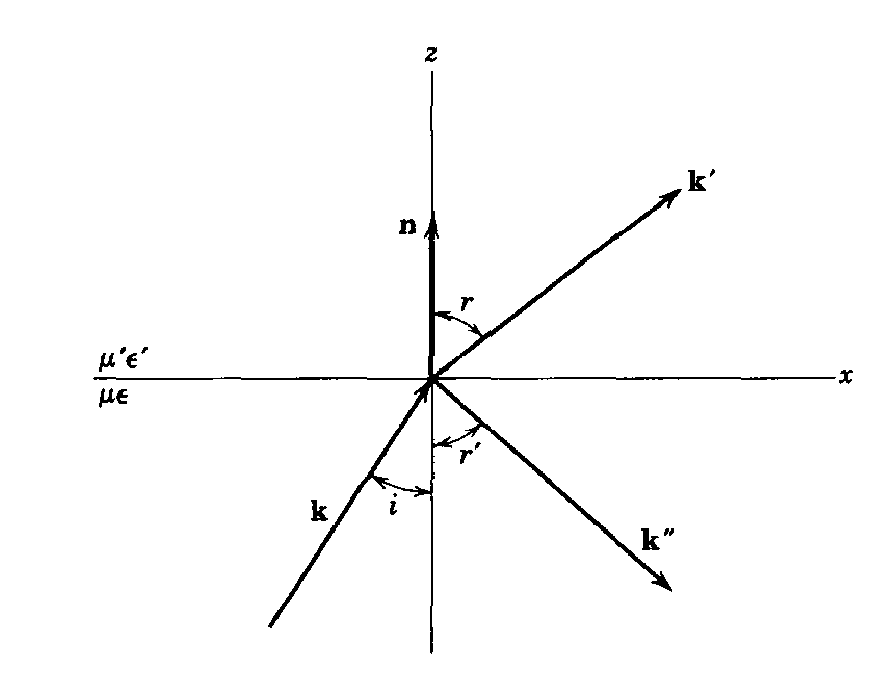
\includegraphics[width=.75\linewidth]{1}
\caption{Propagation of a wave into a medium with a different index of refraction, which gives rise to reflected and refracted waves. The y-axis points into the page for this geometry [\textbf{1}].}
\label{fig:lat}
\end{figure}
Now that we have defined some of the more trivial aspects of our problem, let us derive the Fresnel equations for the situation at hand. Figure 1 demonstrates the geometry we shall be working with; a wave with wave-vector $\mathbf{k}$ is incident on a surface located at $z = 0$ at an angle $\theta_{i}$, which gives rise to a reflected wave $\mathbf{k}''$ at an angle $\theta_{r'}$ and a refracted wave $\mathbf{k}'$ at an angle $\theta_{r}$. Furthermore, we shall restrict our attention to two special cases of linearly polarized light. In the first of these, the electric field oscillates in a plane that is parallel to the plane of incidence, defined as the plane formed by all three wave rays (i.e. the z-x plane in the figure above). Conversely, the magnetic field oscillates in a plane that is orthogonal to the plane of incidence, as can be seen from Eq.(\ref{B}); such a wave is known as a Transverse Magnetic (TM) wave, or p-wave. When the electric field oscillates in a plane that is orthogonal to the plane of incidence, this wave is called a Transverse Electric (TE) wave, or s-wave. Note that we are intentionally leaving out more complicated behavior such as elliptically polarized light for the sake of brevity. \\

Using the superposition principle, we can imagine each of the two regions $\mu \epsilon$ and $\mu' \epsilon'$ as being composed of a combination of forward-moving and backward-moving waves. In the $\mu \epsilon$ region we have the following two waves:
\begin{equation}
\mathbf{E}(\mathbf{r}, t) = \mathbf{E}_{0} e^{i (\mathbf{k} \cdot \mathbf{r} - \omega t)}
\end{equation}
\begin{equation}
\mathbf{E}''(\mathbf{r}, t) = \mathbf{E}_{0}'' e^{i (\mathbf{k}'' \cdot \mathbf{r} - \omega t)}
\end{equation}
\noindent
whereas in the $\mu' \epsilon'$ region we have:
\begin{equation}
\mathbf{E}'(\mathbf{r}, t) = \mathbf{E}_{0}' e^{i (\mathbf{k}' \cdot \mathbf{r} - \omega t)}
\end{equation}
\noindent
Joining all three equations at the interface then gives:
\begin{equation}\label{superp}
\mathbf{E}_{0} e^{i (\mathbf{k} \cdot \mathbf{r} - \omega t)} + \mathbf{E}_{0}'' e^{i (\mathbf{k}'' \cdot \mathbf{r} - \omega t)} = \mathbf{E}_{0}' e^{i (\mathbf{k}' \cdot \mathbf{r} - \omega t)}
\end{equation}
\noindent
Since the frequency is decided at the source, it is the same for all three waves. This leads to the three relations:
\begin{equation}\label{k1}
|\mathbf{k}| = |\mathbf{k}''| = \omega \sqrt{\mu \epsilon}
\end{equation}
\begin{equation}\label{k2}
|\mathbf{k}'| = \omega \sqrt{\mu' \epsilon'}
\end{equation}
\noindent
From Eq.(\ref{superp}) and from the fact that the boundary conditions must hold for all $\mathbf{r}$ and $t$, we see that the arguments of the exponents must all be equal at $z = 0$. Notice how this is happens because the time-dependence is confined to a $e^{-i \omega t}$ harmonic. And so, at $z = 0$ we have the following conditions:
\begin{equation}
\mathbf{k} \cdot \mathbf{r} =  \mathbf{k}'' \cdot \mathbf{r} = \mathbf{k}' \cdot \mathbf{r}
\end{equation}
\noindent
This implies:
\begin{equation}
|k||r| \cos \theta_{i} = |k''||r| \cos \theta_{r'} \hspace{10mm} \rightarrow \hspace{10mm}\theta_{i} = \theta_{r'}
\end{equation}
\noindent
We have thus recovered the law of reflection, demonstrating the fact that all three wave rays lay in the plane of incidence. We may now eliminate the y-components of the scalar products given above and keep only the $k_{x}$ components so that $k_{x} = k_{x}'' = k_{x}'$. This gives:
\begin{equation}
k \sin \theta_{i} = k'' \sin \theta_{r'} = k' \sin \theta_{r}
\end{equation}
\noindent
so that:
\begin{equation}\label{snell}
k \sin \theta_{i} = k' \sin \theta_{r}
\end{equation} 
\noindent
which is a re-statement of Snell's law, as can be seen by using Eq.(\ref{index}), Eq.(\ref{k1}), and Eq.(\ref{k2}). Together, the laws of reflection and refraction dictate the kinematic properties of wave propagation. The \textit{dynamic} properties are dictated by the interface, which we will now examine. The standard boundary conditions of the Maxwell equations state:
\begin{equation}
[ \epsilon (\mathbf{E}_{0} + \mathbf{E}_{0}'') - \epsilon' \mathbf{E}_{0}' ] \cdot \mathbf{n} = 0
\end{equation}
\begin{equation}
[ \mathbf{k} \times \mathbf{E}_{0} + \mathbf{k}'' \times \mathbf{E}_{0}'' - \mathbf{k}' \times \mathbf{E}_{0}' ] \cdot \mathbf{n} = 0
\end{equation}
\begin{equation}
(\mathbf{E}_{0} + \mathbf{E}_{0}'' - \mathbf{E}_{0}' ) \times \mathbf{n} = 0
\end{equation}
\begin{equation}
\left[ \frac{1}{\mu} ( \mathbf{k} \times \mathbf{E}_{0} + \mathbf{k}'' \times \mathbf{E}_{0}'' ) - \frac{1}{\mu'} ( \mathbf{k}' \times \mathbf{E}_{0}') \right] \times \mathbf{n} = 0
\end{equation}
\noindent
Notice how we have eliminated $\mathbf{B}$ through Eq.(\ref{B}). The first two of these equations state that the components of the electric and magnetic fields that are orthogonal to the interface experience a discontinuity and continuity at the interface, respectively; the latter two state that the parallel components of the electric and magnetic fields are continuous and discontinuous at the interface instead. Lets begin applying these boundary conditions to the case of a TM wave. The first condition yields:
\begin{equation}
\epsilon (E_{0} \sin \theta_{i} + E_{0}'' \sin \theta_{r'} ) = \epsilon' E_{0}' \sin \theta_{r}
\end{equation}
\noindent
Using Snell's law and the law of reflection then gives:
\begin{equation}
\sqrt{ \frac{\mu' \epsilon'}{\mu \epsilon} } (E_{0} + E_{0}'' ) = \frac{\epsilon'}{\epsilon} E_{o}'
\end{equation}
\noindent
This can be rearranged to obtain:
\begin{equation}\label{bc1}
\sqrt{ \frac{\epsilon}{\mu} } (E_{0} + E_{0}'' ) = \frac{\epsilon'}{\mu'} E_{o}'
\end{equation}
\noindent
The second boundary condition gives nothing since there are no components of the magnetic fields that are perpendicular to the interface. The third boundary condition imposes restrictions on the parallel components of the electric field and so:
\begin{equation}
-E_{0} \cos \theta_{i} + E_{0}'' \cos \theta_{r'} = -E_{0}' \cos \theta_{r} 
\end{equation}
\noindent
Once again, the law of reflection simplifies this to:
\begin{equation}\label{bc2}
( E_{0} - E_{0}'' ) \cos \theta_{i} = E_{0}' \cos \theta_{r} 
\end{equation}
\noindent
Lastly, the fourth boundary condition merely reproduces Eq.(\ref{bc1}). We now proceed to solve Eq.(\ref{bc1}) and Eq.(\ref{bc2}) for the ratios $E_{0}'' / E_{0}$ and $E_{0}' / E_{0}$, otherwise known as the reflection and transmission coefficients [\textbf{2}]:
\begin{equation}
r \equiv \frac{E_{0}''}{E_{0}} = \frac{ \frac{\mu}{\mu'} n'^{2} \cos \theta_{i} - n \sqrt{ n'^{2} - n^{2} \sin^{2} \theta_{i}}} {\frac{\mu}{\mu'} n'^{2} \cos \theta_{i} + n \sqrt{ n'^{2} - n^{2} \sin^{2} \theta_{i}}}
\end{equation}
\begin{equation}
t \equiv \frac{E_{0}'}{E_{0}} = \frac{2 n n' \cos \theta_{i}}{\frac{\mu}{\mu'} n'^{2} \cos \theta_{i} + n \sqrt{ n'^{2} - n^{2} \sin^{2} \theta_{i}}}
\end{equation}
\noindent
In this paper we will only consider non-magnetic materials for which $\mu = \mu_{0}$ which immediately yields $\mu / \mu' = 1$. Furthermore, the relation $n \sqrt{ n'^{2} - n^{2} \sin^{2} \theta_{i}} = n n' \cos \theta_{r}$ allows us to simplify these expressions to:
\begin{equation}\label{fresnel1}
r_{p} = \frac{ n_{f} \cos \theta_{i} - n_{i} \cos \theta_{f} }{ n_{f} \cos \theta_{i} + n_{i} \cos \theta_{f}}
\end{equation}
\begin{equation}
t_{p} = \frac{ 2 n_{i} \cos \theta_{i} }{ n_{f} \cos \theta_{i} + n_{i} \cos \theta_{f}}
\end{equation}
\noindent
In these expression we have re-labeled $n, n' \rightarrow n_{i}, n_{f}$ and $\theta_{i}, \theta_{r} \rightarrow \theta_{i}, \theta_{r}$ for clarity. The $p$ subscript denotes a p-wave (i.e. a TM wave). Similar calculations for an s-wave give the following relations:
\begin{equation}
r_{s} = \frac{ n_{i} \cos \theta_{i} - n_{f} \cos \theta_{f} }{ n_{i} \cos \theta_{i} + n_{f} \cos \theta_{f}}
\end{equation}
\begin{equation}\label{fresnel2}
t_{s} = \frac{ 2 n_{i} \cos \theta_{i} }{ n_{i} \cos \theta_{i} + n_{f} \cos \theta_{f}}
\end{equation}
\noindent
Equations (\ref{fresnel1} - \ref{fresnel2}) constitute the core of our theory, and we shall use them to derive the behavior of light as it propagates through multiple interfaces.

\section{The Transfer Matrix Method}

Having derived the Fresnel equations, our final step is to generalize them for the case where multiple dielectric interfaces are present. We imagine a scenario similar to Figure 1 but with $N$ layers of different thicknesses $d_{j}$ and indices of refraction $n_{j}$ stacked along the z-axis so that they lay parallel to the y-x plane. This means that the dielectric layers can be organized as follows:
\begin{align}\label{layers}
n(z) =& n_{0}, \hspace{10mm} z < z_{0}                  \nonumber \\
	  & n_{1}, \hspace{10mm} z_{0} < z < z_{1}           \nonumber \\
 	  & n_{2}, \hspace{10mm} z_{1} < z < z_{2}            \nonumber \\
 	  & \vdots                                             \nonumber \\ 	
 	  & n_{N}, \hspace{10mm} z_{N - 1} < z                  \nonumber \\	 
\end{align}
\noindent
From this geometry, it is easy to see that the z-component of $\mathbf{k}$ in each layer becomes $k_{z j} = (2 \pi n_{j} / \lambda_{0}) \cos \theta_{j}$ since, as before, the wave rays are confined to the plane of incidence. Let us now consider the total electric field of a TE (s-wave) within each individual layer, as s-waves tend to satisfy simpler boundary conditions. The superposition principle allows us to once again decompose $\mathbf{E}(\mathbf{r}, t)$ into different components; one moving forward in the positive z-direction, and another moving backwards in the -z-direction [\textbf{3}][\textbf{4}]:
\begin{align}
E(\mathbf{r}, t)  &=  E_{F} e^{ i ( \mathbf{k}_{F} \cdot \mathbf{r} - \omega t) } + E_{B} e^{ i ( \mathbf{k}_{B} \cdot \mathbf{r} - \omega t) }          \nonumber \\
   	              &= E_{F} e^{ i ( k_{x} x + k_{zj} z - \omega t) } + E_{B} e^{ i ( k_{x} x - k_{zj} z - \omega t) }           \nonumber \\
             	  &=  E_{F} e^{ i k_{zj} z } + E_{B} e^{ -i  k_{zj} z }                                   
\end{align}
\noindent
In the last line we absorbed $e^{ i k_{x} x }$ into the complex amplitudes and dropped the time dependence for clarity. We can recast this equation into a more illuminating form if we consider how the state of the light beam changes as it interacts with each layer $j$:
\begin{align}\label{system2}
E_{F}' = E_{F} e^{ i k_{zj} z }  \nonumber \\
E_{B}' = E_{B} e^{ -i  k_{zj} z }
\end{align}
\noindent
Interestingly enough, this resembles a two-state matrix equation of the form:
\begin{equation}
E' = T_{j} E
\end{equation}
\noindent
for some matrix $T_{j}$. Thus, as a wave propagates within a material of thickness $d_{j}$, the corresponding propagation matrix can be obtained through inspection of Eqs.(\ref{system2}):
\begin{equation}\label{Tj}
T_{j} = 
\begin{pmatrix}
	\exp i k_{zj}d_{j} & 0 \\
	0 & \exp - i k_{zj}d_{j}
\end{pmatrix}  = 
\begin{pmatrix}
	\exp i \Phi_{j} & 0 \\
	0 & \exp - i \Phi_{j}
\end{pmatrix}
\end{equation}
\noindent
where we have defined the phase angle as $\Phi_{j} = k_{zj}d_{j}$. As helpful as the $T_{j}$ matrix is, it does not provide the entire picture. We must now investigate how the state of a light wave changes as it passes \textit{through} an interface. The difference can be subtle, so the reader is advised to give is some thought. As was the case for wave reflection and refraction, boundary conditions will once again dictate the dynamics of our system. Since we are dealing with s-waves, the relevant boundary conditions are those for tangential $\mathbf{E}$ and $\mathbf{B}$, which we already acquired in the previous section:
\begin{equation}
E_{Fi} + E_{Bi} = E_{Fj} + E_{Bj} \nonumber
\end{equation}
\begin{equation}
n_{i} \cos \theta_{i} (E_{Fi} - E_{Bi}) = n_{j} \cos \theta_{j} (E_{Fj} - E_{Bj})
\end{equation}
\noindent
The difference in the indices between the left-hand and right-hand sides explicitly demonstrates the propagation of light through an interface. In matrix form these equations read:
\begin{equation}
\begin{pmatrix}
		1 & 1 \\
	n_{i} \cos \theta_{i} & - n_{i} \cos \theta_{i}
\end{pmatrix} 
\begin{pmatrix}
	E_{Fi}  \\
    E_{Bi}
\end{pmatrix} =
\begin{pmatrix}
	1 & 1 \\
	n_{j} \cos \theta_{j} & - n_{j} \cos \theta_{j}
\end{pmatrix} 
\begin{pmatrix}
	E_{Fj}  \\
	E_{Bj}
\end{pmatrix}
\end{equation}
\noindent
Rearranging this expression yields:
\begin{equation}
\begin{pmatrix}
		E_{Fj}  \\
		E_{Bj}
\end{pmatrix} =
\begin{pmatrix}
		1 & 1 \\
		n_{j} \cos \theta_{j} & - n_{j} \cos \theta_{j}
\end{pmatrix}^{-1}
\begin{pmatrix}
	1 & 1 \\
	n_{i} \cos \theta_{i} & - n_{i} \cos \theta_{i}
\end{pmatrix}  
\begin{pmatrix}
		E_{Fi}  \\
		E_{Bi}
\end{pmatrix} \nonumber
\end{equation}
\begin{equation}
\begin{pmatrix}
		E_{Fj}  \\
		E_{Bj}
\end{pmatrix} =
	 T_{j}^{-1} T_{i}
\begin{pmatrix}
		E_{Fi}  \\
		E_{Bi}
\end{pmatrix} = 
    T_{ji}
\begin{pmatrix}
	E_{Fi}  \\
	E_{Bi}
\end{pmatrix}
\end{equation}
\noindent
The transfer matrix $T_{ji}$ is now trivial to find. The end result is:
\begin{equation}\label{Tji}
T_{ji} = \frac{1}{t_{ji}}
\begin{pmatrix}
		1 & r_{ji} \\
		r_{ji} & 1
\end{pmatrix}
\end{equation}
\noindent
Evidently, the elements of $T_{ji}$ are nothing but the Fresnel coefficients we calculated in the previous section. Combining this interface matrix with the layer-propagation matrix Eq.(\ref{Tj}) gives the \textit{total} transfer matrix of our system $T$. For an arbitrary amount of layers, $T$ is obtained through ordinary matrix multiplication of each individual element:
\begin{equation}
T = T_{N(N-1)} T_{N-1} \hdots T_{32} \hspace{1mm} T_{2} \hspace{1mm} T_{21} \hspace{1mm} T_{1} \hspace{1mm} T_{10}
\end{equation}
\noindent
The order of these matrices is to be noted, as this configuration gives the total output from some initial input. For example, reversing this order result in the converse, which is to say:
\begin{equation}
\begin{pmatrix}
	E_{F}(z_{0})  \\
	E_{B}(z_{0})
\end{pmatrix} =
\begin{pmatrix}
	T_{11} & T_{12} \\
	T_{21} & T_{22}
\end{pmatrix}  
\begin{pmatrix}
	E_{F}(z_{N - 1})  \\
	0
\end{pmatrix} \nonumber
\end{equation}
\noindent
Here we are relating the electric fields in the first layer to those in the last layer through a reversed $T$ matrix. Furthermore, we are also assuming that there are no incoming waves from the $N - 1$ layer so that the backwards-traveling wave is zero. We can solve this system of equations for the ratios of reflected-to-incident and transmitted-to-incident amplitudes; these are merely the reflecting and transmission amplitudes:
\begin{equation}
r = \frac{T_{21}}{T_{11}}  \hspace{20mm}   t = \frac{1}{T_{11}}
\end{equation}
\noindent
Our quantities of interest are the reflected and transmitted power, which are easily obtained from the Poynting vector. For convenience we simply state these well-know results [\textbf{1}]:
\begin{equation}\label{R}
R = |r|^{2}
\end{equation}
\begin{equation}
T_{p} = |t|^{2} \frac{  \mathrm{Re} ( n_{f} \cos \theta_{f}^{*} )  }{ \mathrm{Re} ( n_{i} \cos \theta_{i}^{*}  ) }
\end{equation}
\begin{equation}\label{T}
T_{s} = |t|^{2} \frac{  \mathrm{Re} ( n_{f} \cos \theta_{f} )  }{ \mathrm{Re} ( n_{i} \cos \theta_{i} ) }
\end{equation}
\noindent
The reflected power is apparently independent of polarization. Now that we have all the tools required, we can finally make progress and perform some trial computations.

\section{Numerical Implementations of the TMM in Python} 

To put all the tools we developed in the previous sections, we carry out a computation in Python that showcases some of the more significant aspects of the TMM. The following code was adapted from Byrnes module on the TMM [\textbf{5}]. We start by defining a function that distinguishes whether a given wave is traveling forward or backwards in a given medium of complex reflectivity. To achieve this, we perform two \textbf{assert} statements that ensure that both parts of the index of refraction $n$ are positive. As we discussed before, a negative extinction coefficient would lead to exponential growth which we are avoiding. Now, the wave-number in a given layer $k_{z j} = (2 \pi n_{j} / \lambda_{0}) \cos \theta_{j}$ generally points in the direction of propagation in isotropic media, so we can use it to further refine the forward direction criteria. We thus create an \textbf{if} conditional that returns true if the extinction coefficient is above a flotation point value and false otherwise. Since decay points if the forward direction, a positive extinction coefficient is a good metric for this problem:
\lstset{showspaces=false,showstringspaces=false}%
\begin{lstlisting}
def theta_forward(n, theta):

	assert n.real >= 0
	assert n.imag >= 0

	n_cos_theta = n * np.cos(theta)    
	if np.absolute(n_cos_theta.imag) > 100 * EPSILON:
		value = (n_cos_theta.imag > 0)
	else:
		value = (n_cos_theta.real > 0)

return value
\end{lstlisting}
\noindent
We then create a simple function that returns a refracted angle from an incident angle based on Snell's Law Eq.(\ref{snell}) and uses the previous function for forward propagation. If the angle fails to point in the forward direction, this function returns a backwards angle which is simply $(\pi - \theta)$:
\lstset{showspaces=false,showstringspaces=false}%
\begin{lstlisting}
def snells_law(n_1, n_2, theta_1):

	theta_2 = arcsin(n_1 * np.sin(theta_1) / n_2)
	if theta_forward(n_2, theta_2):
		return theta_2
	else:
		return np.pi - theta_2
\end{lstlisting}
\noindent
Moving onward, the next function defines a list of refracted angles within the dielectric structure based on the incident angle on the first layer. The \textbf{if not} conditionals assure that the wave propagates in the forward direction for the first layer \textbf{n\_list[0]} and for the last layer \textbf{n\_list[-1]} as well:
\lstset{showspaces=false,showstringspaces=false}%
\begin{lstlisting}
def snells_law_list(n_list, theta_incident):

	theta_refracted_list = arcsin(n_list[0] 
				* np.sin(theta_incident) / n_list)
	if not theta_forward(n_list[0], theta_refracted_list[0]):
		theta_refracted_list[0] = np.pi - theta_refracted_list[0]
	if not theta_forward(n_list[-1], theta_refracted_list[-1]):
		theta_refracted_list[-1] = np.pi - theta_refracted_list[-1]
	return theta_refracted_list
\end{lstlisting}
\noindent
Now comes the part where we define the reflection amplitudes for s-waves and p-waves directly from the Fresnel equations Eqs.(\ref{fresnel1} - \ref{fresnel2}). The \textbf{if} loops take care of both situations: 
\lstset{showspaces=false,showstringspaces=false}%
\begin{lstlisting}
def reflection_amplitude(polarization, n_i, n_f, theta_i, theta_f):

	if polarization == 's':
		return ((n_i * np.cos(theta_i) - n_f * np.cos(theta_f)) /
			(n_i * np.cos(theta_i) + n_f * np.cos(theta_f)))
	elif polarization == 'p':
		return ((n_f * np.cos(theta_i) - n_i * np.cos(theta_f)) /
			(n_f * np.cos(theta_i) + n_i * np.cos(theta_f)))
	else:
		raise ValueError("Polarization must be 's' or 'p'")

def amplitude_r(polarization, n_i, n_f, theta_i, theta_f):

	r = reflection_amplitude(polarization, n_i, n_f, theta_i, theta_f)
	return reflected_power(r)
\end{lstlisting}
\noindent
Similarly, the transmission amplitudes can be computed for s-waves and p-waves as well. The \textbf{amplitude\_r} and \textbf{amplitude\_t} functions serve to return values that can be fed into the computation of the reflected and transmitted power:
\lstset{showspaces=false,showstringspaces=false}%
\begin{lstlisting}
def transmission_amplitude(polarization, n_i, n_f, theta_i, theta_f):

	if polarization == 's':
		return ((2 * n_i * np.cos(theta_i)) / 
			(n_i * np.cos(theta_i) + n_f * np.cos(theta_f)))
	elif polarization == 'p':
		return ((2 * n_i * np.cos(theta_i)) / 
			(n_f * np.cos(theta_i) + n_i * np.cos(theta_f)))
	else:
		raise ValueError("Polarization must be 's' or 'p'")

def amplitude_t(polarization, n_i, n_f, theta_i, theta_f):

	t = transmission_amplitude(polarization, n_i, n_f, theta_i, theta_f)
	return transmitted_power(polarization, t, n_i, n_f, theta_i, theta_f)
\end{lstlisting}
\noindent
It is now straightforward to define functions that return the \textbf{reflected\_power} and the \textbf{transmitted\_power} functions based on Eqs.(\ref{R} - \ref{T}):
\lstset{showspaces=false,showstringspaces=false}%
\begin{lstlisting}
def reflected_power(r):

	return np.absolute(r)**2

def transmitted_power(polarization, t, n_i, n_f, theta_i, theta_f):

	if polarization == 's':
		return np.absolute(t**2) * (((n_f * np.cos(theta_f)).real) 
			/ (n_i * np.cos(theta_i)).real)
	elif polarization == 'p':
		return np.absolute(t**2)
			*(((n_f * np.conj(np.cos(theta_f))).real) 
			/ (n_i * np.conj(np.cos(theta_i))).real)
	else:
		raise ValueError("Polarization must be 's' or 'p'")
\end{lstlisting}
\noindent
Lastly we define a 2 x 2 \textbf{matrix\_array} function which we will use as a template for our transfer matrices:
\lstset{showspaces=false,showstringspaces=false}%
\begin{lstlisting}
def matrix_array(a, b, c, d, dtype=float):

	template_array = np.empty((2,2), dtype=dtype)
	template_array[0,0] = a
	template_array[0,1] = b
	template_array[1,0] = c
	template_array[1,1] = d
	return template_array
\end{lstlisting}
\noindent
At long last, we can piece all the these functions together to build our TMM algorithm. Lets discuss some of its important features. The first block of code defines a series of tests meant to guide a user's inputs. For example, the first \textbf{if} conditional safeguards against the input of more than one incident wavelength or angle, while the second \textbf{if} conditional ensures that the dimensionality of the \textbf{n\_list} and \textbf{d\_list} arrays does not exceed one. Furthermore, it also returns an error if we have more indices of refraction values than dielectric layers and vice-versa. Next come a series of \textbf{assert} statements that verify that the first layer \textbf{d\_list[0]} and the second layer \textbf{d\_list[-1]} are of infinite thickness, and that our incident angle/index of refraction describe physical values: 
\lstset{showspaces=false,showstringspaces=false}%
\begin{lstlisting}
def transfer_matrix_method(polarization, n_list, d_list, theta_incident, 
	wavelength):

	n_list = np.array(n_list)

	d_list = np.array(d_list, dtype=float) 

	if ((hasattr(wavelength, 'size') and wavelength.size > 1)
		or (hasattr(theta_incident,'size') and theta_incident.size>1)):
	raise ValueError("Only 1 wavelength.......")
	if ((n_list.ndim != 1) 
		or (d_list.ndim != 1) 
		or (n_list.size != d_list.size)):
	raise ValueError("Problem with n_list or d_list!")

	assert d_list[0] == d_list[-1] == np.inf
	assert np.absolute((n_list[0]*np.sin(theta_incident)).imag)<100*EPSILON
	assert theta_forward(n_list[0], theta_incident)
\end{lstlisting}
\noindent           
Once all of these checks have passed, we move on to the implementation of the TMM. The first four lines recast our relevant parameters as lists with values for each layer. Afterwards, we create arrays for our reflection and transmission amplitudes \textbf{r\_list} and \textbf{t\_list} and loop then through all layers. Finally, we create two matrix lists \textbf{Transfer1\_list} and \textbf{Transfer2\_list} which are precisely the $T_{j}$ and $T_{ji}$ matrices we defined in Eq.(\ref{Tj}) and Eq.(\ref{Tji}):
\lstset{showspaces=false,showstringspaces=false}%
\begin{lstlisting}
        num_layers = n_list.size

	theta_list = snells_law_list(n_list, theta_incident)

	k_list = 2 * np.pi * n_list * np.cos(theta_list) / wavelength

	phase_angle = k_list * d_list

	r_list = np.zeros((num_layers, num_layers), dtype=complex)
	t_list = np.zeros((num_layers, num_layers), dtype=complex) 
	for i in range(num_layers-1):
		r_list[i,i+1] = reflection_amplitude(polarization, n_list[i],
   			        n_list[i+1],theta_list[i], theta_list[i+1])
		t_list[i,i+1]=transmission_amplitude(polarization, n_list[i], 
		                n_list[i+1],theta_list[i], theta_list[i+1])

	Transfer1_list = np.zeros((num_layers, 2, 2), dtype=complex)
	for i in range(1, num_layers-1):
		Transfer1_list[i] = (1/t_list[i,i+1]) * np.dot(
			matrix_array(np.exp(-1j * phase_angle[i]), 
			     0, 0, np.exp(1j * phase_angle[i]),dtype=complex),
			matrix_array(1, r_list[i,i+1], r_list[i,i+1],
			     1, dtype=complex))

	Transfer2_list = matrix_array(1, 0, 0, 1, dtype=complex)
	for i in range(1, num_layers-1):
		Transfer2_list = np.dot(Transfer2_list, Transfer1_list[i])

	Transfer2_list = np.dot(matrix_array(1,r_list[0,1], r_list[0,1], 1,
		dtype=complex)/t_list[0,1], Transfer2_list)
\end{lstlisting}
\noindent
Finally, we construct the reflection and transmission amplitudes/powers from our matrices and then end the algorithm by returning values for all variables. An extra function that is included is the \textbf{unpolarized} function which, as its name states, returns the reflected/transmitted powers for unpolarized light by averaging the s-waves with the p-waves: 
\lstset{showspaces=false,showstringspaces=false}%
\begin{lstlisting}
	r = Transfer2_list[1,0]/Transfer2_list[0,0]
	t = 1/Transfer2_list[0,0]

	R = reflected_power(r)
	T = transmitted_power(polarization, t,
		n_list[0], n_list[-1], theta_incident, theta_list[-1])

	return {'r': r, 't': t, 'R': R, 'T': T,
	'k_list': k_list, 'theta_list': theta_list,
	'polarization': polarization, 'n_list': n_list, 'd_list': d_list, 
	'theta_incident': theta_incident, 'wavelenght': wavelength}

def unpolarized(n_list, d_list, theta_incident, wavelength):

	s_data = transfer_matrix_method('s', n_list, d_list,
	 theta_incident, wavelength)
	p_data = transfer_matrix_method('p', n_list, d_list,
	 theta_incident, wavelength)
	R = (s_data['R'] + p_data['R']) / 2.
	T = (s_data['T'] + p_data['T']) / 2.
	return {'R': R, 'T': T}
\end{lstlisting}

\newpage

\section{Conclusion}

The transfer matrix method outlined in this paper is a deceptively simple yet versatile instrument that has proven to be indispensable in a diverse array of scientific fields. Although we focused on a narrow range of its applications, we nevertheless arrived at conclusions that seemed to be acquired almost out of sheer luck. Indeed it is quite surprising that this method works at all, given the complicated interactions that take place between light and matter. Please refer to the accompanying Jupyter Notebook for a more detailed overview of some of the computations that the TMM can perform.  

\begin{thebibliography}{1}
	
\bibitem{1} J. Jackson, \textit{Classical Electrodynamics} (John Wiley \& Sons, Inc., 1999).
	
\bibitem{2} E. Hecht, \textit{Optics} (Pearson, 2002).
	
\bibitem{3} M. Born, and E. Wolf, \textit{Priciples of Optics} (Pergamon Press, 1986).
	
\bibitem{4} M. Claudia Troparevsky, Adrian S. Sabau, Andrew R. Lupini, and Zhenyu Zhang, "Transfer-matrix formalism for the calculation of optical response in multilayer systems: from coherent to incoherent interference," Opt. Express 18, 24715-24721 (2010)

\bibitem{5} https://pypi.org/project/tmm/

\end{thebibliography}

\end{document}
